% $Id$
%!TEX TS-program = Arara
% arara: pdflatex
\documentclass[a4paper,11pt,oneside,ngerman]{scrbook}

\usepackage[utf8]{inputenc}
\usepackage[T1]{fontenc}
\usepackage{booktabs}
\usepackage{babel}
\usepackage{graphicx}
\usepackage{csquotes}
\usepackage{paralist}
\usepackage{xcolor}
\usepackage{listings}
%\usepackage{libertine}

\setlength{\parindent}{0pt}
\setlength{\parskip}{0.5em}

\usepackage{microtype}

\usepackage{makeidx} 
\makeindex

\usepackage[flushmargin]{footmisc}


\usepackage{amsmath}
%\usepackage{amssymb} %,amscd,latexsym   
%\usepackage{amsfonts}
%\usepackage{amsthm}


\title{Cryptool}
\author{Cryptool Projekt}

\usepackage{ragged2e} % be_2016-08-04: ragged margin with hyphenation w/ blackbox in index

\newtheorem{definition}{Definition}[section]
\newtheorem{satz}{Satz}[section]
\newenvironment{proof}[1]{\noindent\textbf{Beweis #1} \\}{\hfill$\Box$\par}
\newenvironment{Beweis}[1]{\noindent\textbf{Beweis #1} \\}{\hfill$\Box$\par}
\newenvironment{example}[1]{\noindent\textbf{Beispiel#1}}{}
\newenvironment{remark}[1]{\noindent\textbf{Bemerkung#1}}{}

% Immer als letztes laden, definiert viel um
\usepackage[colorlinks=true,linkcolor=blue,citecolor=blue,urlcolor=black,bookmarksnumbered=true,pdfpagelabels,plainpages=false,hyperfootnotes=false]{hyperref}
\begin{document}


\maketitle


\tableofcontents

% $Id$
% ............................................................................
%      V O R W O R T  und  E I N F � H R U N G (Zusammenspiel Skript-CT) 
% ~~~~~~~~~~~~~~~~~~~~~~~~~~~~~~~~~~~~~~~~~~~~~~~~~~~~~~~~~~~~~~~~~~~~~~~~~~~~


% --------------------------------------------------------------------------
\section*{Preface to the 7th Edition of the CrypTool Script}
\addcontentsline{toc}{section}{Preface to the 7th Edition of the CrypTool Script}

Starting in the year 2000 this script became a part of the 
CrypTool\index{CrypTool} package. It is designed to accompany the program 
CrypTool by explaining some mathematical topics in more detail, 
but still in a way which is easy to understand.

In order to also enable developers/authors to work together independently 
the topics have been split up and for each topic an extra chapter has been 
written which can be read on its own. The later editorial work in TeX added 
cross linkages between different sections and footnotes describing where you
can find the according functions within the CrypTool\index{CrypTool} 
program \hyperlink{appendix-menutree}{(see menu tree in appendix A).}
% in \ref{s:appendix-menutree}   AUFPASSEN, DASS nichts doppelt !!
% \hypertarget{appendix-menutree}{}\label{s:appendix-menutree}
Naturally there are many more interesting topics in mathematics and
cryptography which could be discussed in greater depth -- therefore this
is only one of many ways to do it.

\vspace{12pt}
The rapid spread of the Internet has also lead to intensified research in the
technologies involved, especially within the area of cryptography where a good
deal of new knowledge has arisen.

This edition of the script adds some topics, but mainly updates areas (e.g. the
summaries of topical research areas):
\vspace{-7pt}
\begin{itemize}
  \item the search for the largest prime numbers (generalized Mersenne 
        and Fermat primes) \\ 
%        and Fermat primes, ``M-40'') 
	(chap. \ref{spezialzahlentypen}, \ref{zahlentyp_mersenne}), 
  \item the factorisation of big numbers (RSA-200)\index{RSA-200} 
        (chap. \ref{RSA-200}),
  \item progress in cryptanalysis of hash algorithms 
        (chap. \ref{collision-attacks-against-sha-1}),
  \item progress in ideas for new crypto methods (RSA successor) 
        (chap. \ref{xxxxxxxxxBrute-force-gegen-Symmetr})\index{xxxxxxxxxxxxxxxx} and
  \item a list, in which movies or novels cryptography or number theory has a 
        major role (see appendix \ref{s:appendix-movies}).
\end{itemize}

\vspace{12pt}
The first time the document was delivered with CrypTool\index{CrypTool} 
was in version 1.2.01. Since then it has been expanded and revised in almost every 
new version of CrypTool (1.2.02, 1.3.00, 1.3.02, 1.3.03, 1.3.04 and now 1.3.10).

I'd be more than happy if this also continues in the further open-source
versions of CrypTool\index{CrypTool}.

I am deeply grateful to all the people helping with their impressive
commitment who have made this global project so successful. Especially I would
like to acknowledge the English language proof-reading of this script version
done by Richard Christensen and Lowell Montgomery.

I hope that many readers have fun with this script and that they get 
out of it more interest and greater understanding of this modern but 
also very ancient topic.
\\


Bernhard Esslinger

Frankfurt (Germany), June 2005



% --------------------------------------------------------------------------
\newpage
\section*{Introduction -- How do the Script and the Program Play together?}  \addcontentsline{toc}{section}{Introduction -- How do the Script and the Program Play together?}


\textbf{This script}

This document is delivered together with the program CrypTool\index{CrypTool}.
\par \vskip + 3pt

The articles in this script are largely self-contained and
can also be read independently of CrypTool\index{CrypTool}.

Chapters  \ref{Chapter_ModernCryptography} (Modern Cryptography) and 
\ref{Chapter_EllipticCurves} (Elliptic Curves) require a deeper knowledge
in mathematics, while the other chapters should be understandable with a 
school leaving certificate.

The authors
% \hyperlink{appendix-authors}{(authors)}
% in \ref{s:appendix-authors}
% \hypertarget{appendix-authors}{}\label{s:appendix-authors}
have attempted to describe cryptography for a broad 
audience -- without being mathematically incorrect. We believe that this
didactical pretension is the best way to promote the awareness for IT
security and the readiness to use standardised modern cryptography.
\par \vskip + 15pt


\textbf{The program CrypTool\index{CrypTool}}

CrypTool\index{CrypTool} is a program with an extremely comprehensive online
help enabling you to use and analyse cryptographic procedures within a
unified graphical user interface.\par \vskip + 3pt

CrypTool\index{CrypTool} was developed during the end-user awareness program
at Deutsche Bank in order to increase employee awareness of IT security and provide them with
a deeper understanding of the term security.
A further aim has been to enable users to understand the cryptographic
procedures. In this way, using CrypTool
as a reliable reference implementation of the various encryption procedures
(because of using the industry-proven Secude library\index{SECUDE IT Security}),
you can test the encryption implemented in other programs. \par \vskip + 3pt

CrypTool\index{CrypTool} is currently been used for 
training in companies and teaching at school and universities, and
moreover several universities are helping to further develop the project.
\par \vskip + 15pt


\textbf{Acknowledgment}

At this point I'd like to thank explicitly six people who particularly 
contributed to CrypTool\index{CrypTool}. Without their special talents
 and engagement CrypTool would not be what it is today:
\vspace{-7pt}
\begin{itemize}
   \item Mr.\ Henrik Koy
   \item Mr.\ J\"org-Cornelius Schneider
   \item Dr.\ Peer Wichmann
   \item Prof. Dr. Claudia Eckert,  Mr.\ Thomas Buntrock and Mr.\ Thorsten Clausius.
\end{itemize}
Also I want to thank all the many people not mentioned here for their 
hard work (mostly carried out in their spare time).
\\

Bernhard Esslinger

Frankfurt (Germany), June 2005

% Local Variables:
% TeX-master: "../script-en.tex"
% End:


% $Id$
% ............................................................................
%             V E R S C H L U E S S E L U N G S V E R F A H R E N
% ~~~~~~~~~~~~~~~~~~~~~~~~~~~~~~~~~~~~~~~~~~~~~~~~~~~~~~~~~~~~~~~~~~~~~~~~~~~~

\begin{bibunit}[babalpha] %% alpha: Chapter bibliography shows authors abbreviation


% HACK to fix warning "destination with the same identifier .. has already been used, ...":
% REMOVED, because it caused missing index entries
%\makeatletter \renewcommand{\thepage}{~\csname @arabic\endcsname \c@page} \makeatother

%%%% Old naming: \hypertarget{Kapitel_1}{}
\hypertarget{Chapter_EncryptionSecDefinitions}{}

\chapter{Sicherheits-Definitionen und Verschl�sselungsverfahren}
\label{Chapter_EncryptionSecDefinitions}
(\hyperlink{author_Bernhard-Esslinger}{Bernhard Esslinger},
 \hyperlink{author_Joerg-Cornelius-Schneider}{J�rg-Cornelius Schneider},
 Mai 1999; Updates: Dez. 2001, Feb. 2003, Juni 2005, Juli 2007, Jan. 2010, M�rz 2013, Aug. 2016)

Dieses Kapitel soll einen eher beschreibenden Einstieg bieten und die
Grundlagen ohne Verwendung von allzu viel Mathematik vermitteln.

Sinn der Verschl�sselung \index{Verschl�sselung} ist es, Daten so zu
ver�ndern, dass nur ein autorisierter Empf�n\-ger in der Lage ist,
den Klartext zu rekonstruieren. Das hat den Vorteil, dass verschl�sselte
Daten offen �bertragen werden k�nnen und trotzdem keine Gefahr besteht,
dass ein Angreifer die Daten unberechtigterweise lesen kann. Der
autorisierte Empf�nger ist im Besitz einer geheimen Information, des
sogenannten Schl�ssels, die es ihm erlaubt, die Daten zu entschl�sseln,
w�hrend sie jedem anderen verborgen bleiben.\footnote{%
  Nat�rlich kann ein Angreifer trotzdem die Verbindung st�ren oder
  Metadaten (wie wer mit wem kommuniziert) abgreifen.
}%\par \vskip + 3pt

Zur Erl�uterung verwenden wir im Folgenden die Begriffe aus der
Abbildung \ref{cm_Generic-Notations-when-Encrypting}:
\begin{figure}[ht]
\begin{center}
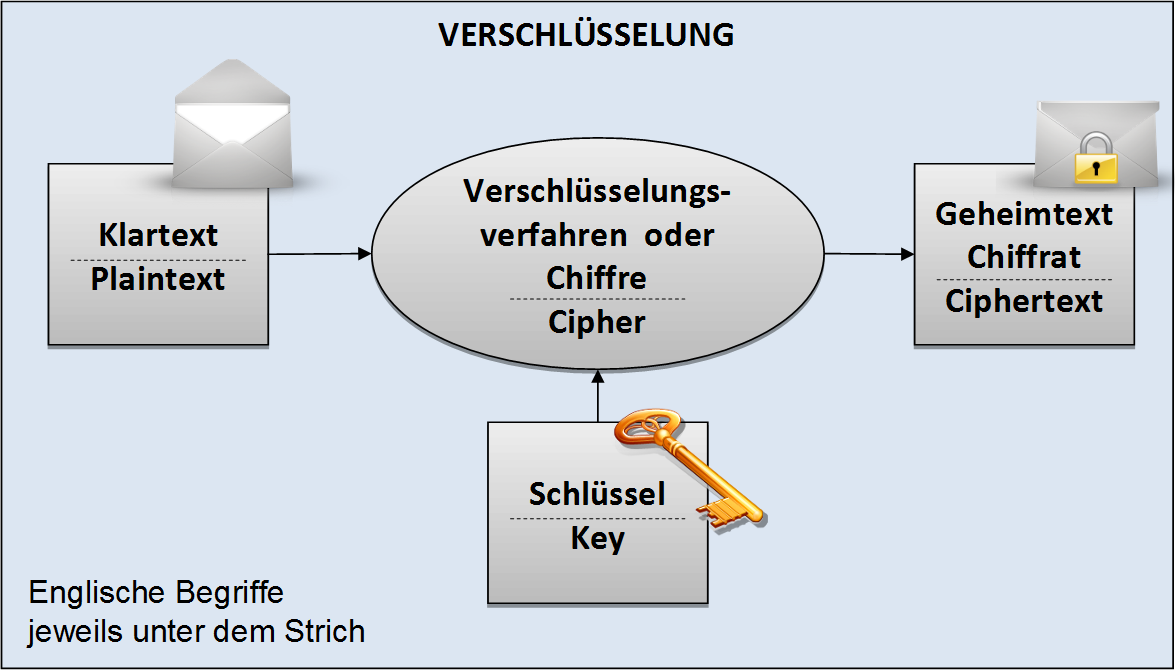
\includegraphics[scale=0.7]{figures/Generic-Notation-Encryption_de.png}
\caption{�bliche Bezeichnungen bei der Verwendung von Verschl�sselungsverfahren} 
\label{cm_Generic-Notations-when-Encrypting}
\end{center}
\end{figure}



% --------------------------------------------------------------------------
\newpage

\begin{ctsquote}
Erkl�re es mir, ich werde es vergessen.\\
Zeige es mir, ich werde es vielleicht behalten.\\
Lass es mich tun, und ich werde es k�nnen.
\caption{Indisches Sprichwort}
\end{ctsquote}


% --------------------------------------------------------------------------
\hypertarget{cm_Section_Security_Definitions}{}
\section{Sicherheits-Definitionen und Bedeutung der Kryptologie}
\label{cm_Section_Security_Definitions}
\index{Sicherheits-Definitionen}

Zuerst erkl�ren wir, wie die Sicherheit von Kryptosystemen definiert wird.

\noindent Moderne Kryptographie basiert vor allem auf mathematischer Theorie und
Computer-Praxis. Beim Design kryptographischer Algorithmen werden Annahmen
zur Schwierigkeit von Berechnungen so gemacht, so dass sich solche Verfahren
in der Praxis von einem Angreifer nur schwer brechen lassen.

\vskip +3pt
Die zwei Hauptnotationen in der Literatur definieren Sicherheit in
Abh�ngigkeit von den M�glichkeiten des Angreifers (vgl. z.B.
{\em Contemporary Cryptography} \cite{Oppliger2011}):

\begin{itemize}

\item {\bf Berechenbare, bedingte oder praktische Sicherheit}\\
  Ein Verschl�sselungsverfahren ist {\em berechenbar} sicher, wenn es (obwohl
  es theoretisch m�glich ist, es zu brechen) selbst mit den besten bekannten
  Verfahren nicht gebrochen werden kann. Theoretische Fortschritte (z.B.
  Verbesserungen bei den Algorithmen zur Faktorisierung) und schnellere
  Computer erfordern, dass dies st�ndig angepasst wird. 

  Selbst wenn man den besten bekannten Algorithmus zum Brechen benutzt, wird
  man so viele Ressourcen brauchen (z.B. 1.000.000 Jahre), dass das Kryptosystem
  sicher ist.

  Daher basiert dieses Konzept auf Annahmen �ber die begrenzte Rechenkraft des
  Angreifers und auf dem aktuellen Stand der Wissenschaft.

\item {\bf Informations-theoretische oder unbedingte Sicherheit}\\
  Ein Verschl�sselungsverfahren wird als {\em unbedingt} sicher bezeichnet,
  wenn seine Sicherheit gew�hrleistet ist, v�llig unabh�ngig davon, wieviele
  Ressourcen (Zeit, Speicher) der Angreifer hat -- also auch in dem Fall,
  wenn der Angreifer unbegrenzt viele Ressourcen hat, um das
  Verfahren zu brechen. Auch mit unbegrenzt vielen Ressourcen kann der
  Angreifer aus dem Chiffrat keine sinnvollen Informationen gewinnen.

  Es gibt Informations-theoretisch sichere Verfahren, die beweisbar nicht
  gebrochen werden k�nnen, auch nicht mit unendlich viel Rechenkraft -- ein
  Beispiel daf�r ist das {\em One-Time-Pad} (OTP\index{OTP}).

  Da das OTP ein Informations-theoretisch sicheres Verschl�sselungsverfahren
  ist, leitet sich seine Sicherheit schon allein aus der Informationstheorie
  ab -- und ist sicher, auch wenn der Angreifer unbegrenzte Rechenkapazit�ten
  hat. Das OTP weist allerdings einige praktische Nachteile auf (der
  verwendete Schl�ssel darf nur einmal verwendet werden, muss zuf�llig
  gew�hlt werden und mindestens so lang sein wie die zu sch�tzende Nachricht),
  so dass es au�er in geschlossenen Umgebungen, zum Beispiel beim hei�en
  Draht zwischen Moskau und Washington, kaum eine Rolle spielt.%\par \vskip + 3pt

\end{itemize}


\vskip +3pt
\noindent Manchmal werden auch zwei weitere Konzepte verwendet:

\begin{itemize}

\item {\bf Beweisbare Sicherheit}
Dies bedeutet, dass das Brechen eines Kryptosystems mindestens so schwierig ist
wie die L�sung eines bestimmten schwierigen Problems, z.B. die Berechnung des
diskreten Logarithmus, die diskrete Quadratwurzel-Berechnung oder die
Faktorisierung sehr gro�er Zahlen.

Beispiel: Aktuell wissen wir, dass RSA\index{RSA} h�chstens so schwierig
ist wie die Faktorisierung, aber wir k�nnen nicht beweisen, dass es genauso
schwierig ist.
Deshalb hat RSA keine beweisbare Mindest-Sicherheit. Oder in anderen Worten:
Wir k�nnen nicht beweisen, dass wenn das Kryptosystem RSA gebrochen ist, dass
dann auch die Faktorisierung (ein schwieriges mathematisches Problem) gel�st
werden kann.

Das Rabin-Kryptosystem war das erste Kryptosystem, f�r das sich beweisen lie�,
dass es berechenbar �quivalent zu einem harten mathematischen Problem ist.

\item {\bf Ad-hoc-Sicherheit}
Ein kryptographisches System hat diese Sicherheit, wenn es sich nicht lohnt,
es zu versuchen es zu brechen, weil der Aufwand daf�r teurer ist als der Wert
der Daten, die man durch das Brechen erhalten w�rde. Z.B. weil ein Angriff
nicht in einer ausreichend kurzen Zeit erfolgen kann (vgl.
{\em Handbook of Applied Cryptography} \cite{Menezes2001}).

Dies kann z.B. zutreffen, wenn B�rsen-relevante Daten sowieso am
n�chsten Tag ver�ffent"-licht werden und man f�r das Brechen ein Jahr brauchen
w�rde.

\end{itemize}


\vskip +3pt
Bei den heutzutage verwendeten guten Verfahren ist der Zeitaufwand zum Brechen
so hoch, dass sie praktisch nicht gebrochen werden k�nnen. Deshalb kann man
diese Verfahren als (praktisch) sicher ansehen -- aus einer rein auf den
Algorithmus bezogenen Sichtweise.\footnote{%
  Insbesondere seit den Informationen von Edward Snowden\index{Snowden, Edward} gab es
  viele Diskussionen, ob Verschl�sselung sicher ist. In \cite{Esslinger2014} wird das
  Ergebnis einer Evaluierung vorgestellt, auf welche Kryptographie man sich verlassen
  kann -- nach dem heutigen Kenntnisstand.
  Der Artikel untersucht: Welche Krypto-Verfahren k�nnen im Lichte der NSA-Enth�llungen
  noch als sicher gelten? Wo wurden Systeme gezielt geschw�cht? Wie k�nnen wir die
  kryptographische Zukunft sicher gestalten? Wie unterscheiden sich Mathematik und
  Implementierung?
}

\vskip +3pt
\begin{sloppypar}
Grunds�tz"-lich unterscheidet man zwischen symmetrischen
(siehe Kapitel \ref{cm_Section_Symmetric-encryption}) und asymmetrischen
(siehe Kapitel \ref{cm_Section_Asymmetric-encryption})
Verfahren zur Verschl�sse"-lung.
Einen sehr guten �berblick �ber die verschiedenen Verschl�sselungsverfahren
bieten auch die B�cher von Bruce Schneier \cite{Schneier1996} und Klaus Schmeh
\cite{Schm2016}.\footnote{%
  Einen kompakten �berblick, der erkl�rt, was wozu verwendet wird, welche der Verfahren
  sicher sind, wo mit Problemen zu rechnen ist und wo die wichtigen Baustellen f�r die
  absehbare Zukunft liegen incl. des Procederes bei den Standardisierungen finden Sie
  in \cite{Schmidt2016}.
  % TODO Info an ju, dass Schreibweise korr ("s" anh�ngen)
  %%     bei "Bereits 1883 formulierte Auguste Kerckhoff".
  % Dieser Artikel erschien urspr�nglich in c't 01/2016, Seite 174
  % Kryptographie in der IT - Empfehlungen zu Verschl�sselung und Verfahren.
  % Kryptographie ist ein wichtiger Baustein moderner IT � Sicherheit,
  % Vertraulichkeit und Privatsph�re h�ngen davon ab. Der folgende Krypto-Wegweiser
  % gibt einen kompakten �berblick zu den aktuell relevanten Verfahren.
}
\end{sloppypar}

\vskip +3pt
Bevor Verschl�sselungstechnologien mit dem Aufkommen des Internets und der drahtlosen
Kommunikation f�r jedermann zur Verf�gung standen, waren sie schon seit Jahrhunderten
im Gebrauch von Regierungen, Milit�rs und Diplomaten. Welche Seite diese Technologie
besser beherrschte konnte mit Hilfen der Geheimdienste gro�en Einfluss auf die {\bf Politik}
und den Kriegsverlauf nehmen. Auf die Historie geht dieses Buch nur insofern ein, als
in Kapitel \ref{Chapter_PaperandPencil} auch die fr�her benutzten Verfahren vorgestellt
werden. Einen Eindruck, welch entscheidende Bedeutung Kryptologie f�r die M�chtigen
hatte und hat, kann man anhand der beiden folgenden Beispiele bekommen: dem Lehrfilm
\glqq Krieg der Buchstaben\grqq\footnote{%
  Der Film \index{Krieg der Buchstaben} schildert vor dem Hintergrund der Weltpolitik
  von 1900-1945 die Entwicklung der Kryptologie und ihre Bedeutung f�r den
  Kriegsverlauf im ersten (Zimmermann-Depesche) und zweiten Weltkrieg. Ausf�hrlich
  wird -- aus anglo-amerikanischer Sicht -- darauf eingegangen, wie bedeutsam die
  Kryptoanalyse (auf dem Atlantik gegen die Enigma und auf dem Pazifik gegen Purple)
  f�r den Verlauf des zweiten Weltkriegs war.\\
  Siehe \url{http://bscw.schule.de/pub/bscw.cgi/d1269787/Krieg_der_Buchstaben.pdf}.
}
und der Debatte um die sogenannten Krypto-Wars\footnote{%
  Siehe \url{https://de.wikipedia.org/wiki/Crypto_Wars}.\index{Krypto-Wars}
}.
%% Vgl. http://scilogs.spektrum.de/hlf/verschluesselte-hintertuerchen-tag-internet-licht/
%%      http://www.heidelberg-laureate-forum.org/de/2015/08/17/eine-debatte-ueber-die-herausforderungen-einer-datengesteuerten-welt/
%%      http://wwwde.uni.lu/snt/news_events/prof_peter_ryan_gives_lecture_at_heidelberg_laureate_forum
%% Diskussion auf dem 3. Heidelberg Laureate Forum (HLF) am Dienstag, 25. August 2015.


% --------------------------------------------------------------------------
\newpage

\begin{ctsquote}
\glqq Man kann nicht nicht kommunizieren!\grqq 
\caption[Paul Watzlawick]{Paul Watzlawick\footnotemark}\index{Watzlawick, Paul}
\end{ctsquote}
\addtocounter{footnote}{0}\footnotetext{Paul Watzlawick, Janet H. Beavin und Don D. Jackson, \glqq Menschliche Kommunikation. Formen, St�rungen, Paradoxien\grqq, Huber, (c) 2007, Das erste der f�nf pragmatischen Axiome ihrer Kommunikationstheorie.}

% --------------------------------------------------------------------------
\section[Einfl�sse auf Verschl�sselungsverfahren] % Was zw. [..] steht, kommt ins Inhaltsverzeichnis!
{Einfl�sse auf Verschl�sselungsverfahren}

% \nopagebreak
Hier sollen kurz zwei Aspekte von Kryptoverfahren erw�hnt werden, auf die oft nicht fr�h genug eingegangen wird:

\begin{itemize}

\item {\bf Zufallsbasiert}\\
\index{Zufall}
Man kann Algorithmen aufteilen in deterministische\index{deterministisch} und heuristische\index{heuristisch} Verfahren. Meistens lernten Studenten nur deterministische Verfahren kennen, bei denen die Ausgabe eindeutig durch die Eingabe vorgegeben wird. Bei heuristischen Verfahren werden Entscheidungen aufgrund zuf�lliger Werte getroffen. Moderne Verfahren des maschinellen Lernens geh�ren ebenfalls hierzu.

In Kryptoverfahren spielt Zufall eine gro�e Rolle. Immer m�ssen die Schl�ssel zuf�llig gew�hlt werden, so dass zumindest bei der Schl�sselgenerierung~\glqq Zufall\grqq~erzeugt werden muss. Zus�tzlich sind manche Verfahren (vor allem aus der Kryptoanalyse) heuristisch.

\item {\bf Konstanten-basiert}\\
Viele moderne Verfahren (insbesondere Hashverfahren und symmetrische Verschl�sse-lungsverfahren) benutzen numerische Konstanten. Diese sollten nachvollziehbar sein und keine Hintert�ren erm�glichen. Zahlen, die das erf�llen, nennt man im Englischen~\glqq Nichts-im-�rmel\grqq-Zahlen: Nothing-up-my-sleeve number\index{Zahlen!Nothing-up-my-sleeve}.%
\footnote{\url{http://en.wikipedia.org/wiki/Nothing_up_my_sleeve_number}}

\end{itemize}


\newpage
Die folgende Abbildung \ref{cm_Figure_OTP-demo-pictures} soll eine Idee davon vermitteln, dass es nicht m�glich ist, bei einem OTP\index{OTP} den Klartext zu bestimmen (sofern das OTP-Verfahren richtig angewendet wird und alle Schl�ssel gleich wahrscheinlich sind).

In dem Beispiel in der Abbildung ist als Geheimtext ein 8 Zeichen langes Wort gegeben:
\texttt{11 1B 1E 18 00 04 0A 15}.
Es gibt viele sinnvolle Worte aus 8 Buchstaben und zu jedem einen passenden Schl�ssel.
Ein Angreifer kann damit allein nicht bestimmen, welches der richtige Schl�ssel bzw.
welches das richtige Klartext-Wort ist.

Vergleiche auch Abbildung~\ref{fig-bool-otp} in Kapitel \ref{s-bool-bitstr-real-random},
wo ein entsprechendes Text-Beispiel mit SageMath erstellt wird.
\begin{figure}[ht]
\begin{center}
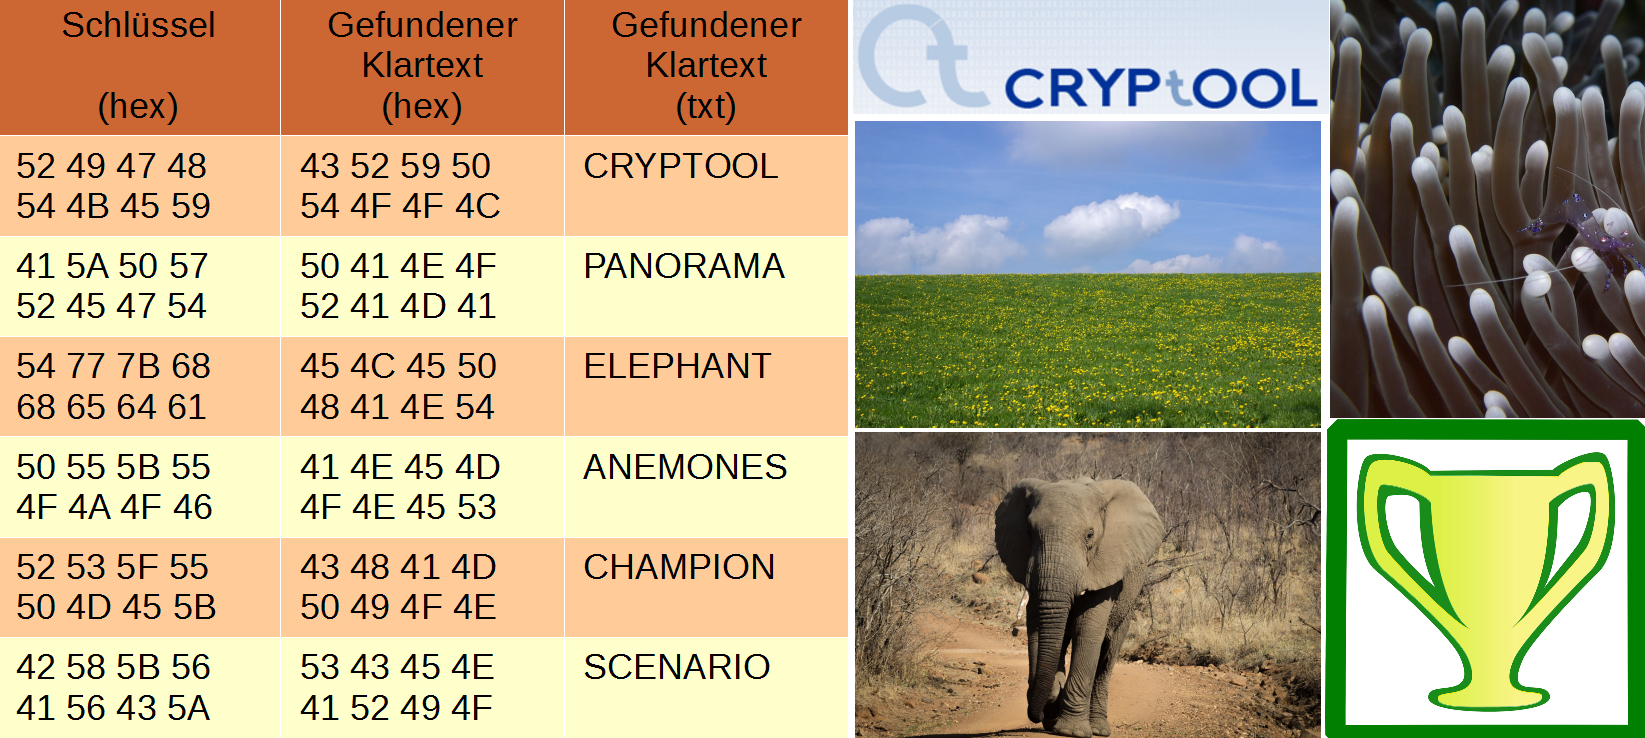
\includegraphics[scale=0.55]{figures/OTP-demo-pictures-de.png}
\caption[Illustration f�r die Informations-theoretische Sicherheit des OTP]
        {Illustration f�r die Informations-theoretische Sicherheit des OTP\footnotemark}
\label{cm_Figure_OTP-demo-pictures}
\end{center}
\end{figure}
\footnotetext{
  Bildquelle: Kostenlose Bilder von \url{https://pixabay.com/}
}





% --------------------------------------------------------------------------
\newpage

\begin{ctsquote}
\glqq Transparenz. Das ist das H�chste, was man sich in einer technologisch hoch entwickelten Gesellschaft erhoffen kann ... sonst wird man einfach nur manipuliert.\grqq 
\caption[Daniel Suarez]{Daniel Suarez\footnotemark}\index{Suarez, Daniel}
\end{ctsquote}
\addtocounter{footnote}{0}\footnotetext{Daniel Suarez, \glqq Darknet\grqq,
            rororo, (c) 2011, Kapitel 5, \glqq Einsichten\grqq, S. 69, Price.}

% --------------------------------------------------------------------------
\section[Symmetrische Verschl�sselung] % Was zwischen [...] steht, kommt ins Inhaltsverzeichnis!
        {Symmetrische Verschl�sselung\footnotemark}
  \footnotetext{% Dieses Prozent ist n�tig, sonst startet die Fu�note mit einem Blank !
    Mit CrypTool~1 ({\bf CT1})\index{CT1} k�nnen Sie �ber das
    Men� {\bf Ver-/Entschl�sseln \textbackslash{} Symmetrisch (modern)} folgende
    modernen symmetrischen Verschl�sselungsverfahren ausf�hren:\\
    IDEA, RC2, RC4, DES (ECB), DES (CBC), Triple-DES (ECB), Triple-DES (CBC),
    MARS (AES-Kandidat), RC6 (AES-Kandidat), Serpent (AES-Kandidat), 
    Twofish (AES-Kandidat),
    Rijndael (offizielles AES-Verfahren)\index{AES}.\\
    Mit CrypTool~2 ({\bf CT2})\index{CT2} k�nnen Sie im Startcenter
    �ber {\bf Vorlagen \textbackslash{} Kryptographie \textbackslash{}
    Modern \textbackslash{} Symmetrisch} folgende modernen symmetrischen
    Verschl�sselungsverfahren ausf�hren:\\ 
    AES, DES, PRESENT, RC2, RC4, SDES, TEA, Triple-DES, Twofish.\\
    In JCrypTool ({\bf JCT})\index{JCT} stehen Ihnen die folgenden
    modernen symmetrischen Verschl�sselungsverfahren zur Verf�gung:\\ 
    AES, Rijndael, Camellia, DES, Dragon, IDEA, LFSR, MARS, Misty1, RC2, RC5,
    RC6, SAFER+, SAFER++, Serpent, Shacal, Shacal2, Twofish.
    }
\label{cm_Section_Symmetric-encryption}

\nopagebreak

Bei der {\em symmetrischen} Verschl�sselung 
\index{Verschl�sselung!symmetrisch} m�ssen Sender und Empf�nger
�ber einen gemeinsamen (geheimen) Schl�ssel verf�gen, den sie vor
Beginn der eigentlichen Kommunikation ausgetauscht haben. Der Sender
benutzt diesen Schl�ssel, um die Nachricht zu verschl�sseln und der
Empf�nger, um diese zu entschl�sseln.\par %\vskip + 3pt

Dies veranschaulicht Abbildung \ref{cm_Figure_Symmetric-Enc_Secret-Key-Enc}:
\begin{figure}[ht]
\begin{center}
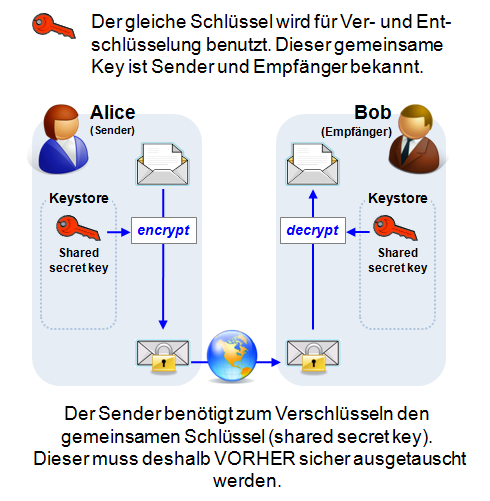
\includegraphics[scale=0.7]{figures/SymmetricEnc_Figure_Chap1_de.png}
\caption{Symmetrische oder Secret-Key-Verschl�sselung} 
\label{cm_Figure_Symmetric-Enc_Secret-Key-Enc}
\end{center}
\end{figure}

Alle klassischen Chiffren sind vom Typ symmetrisch. Beispiele dazu finden Sie
in den CT-Programmen, im Kapitel~\ref{Chapter_PaperandPencil}
(\glqq \nameref{Chapter_PaperandPencil}\grqq)
in diesem Skript oder in \cite{Nichols1996}. 
In diesem Unterkapitel wollen wir jedoch nur die moderneren symmetrischen
Verfahren betrachten.

Vorteile von symmetrischen Algorithmen sind die hohe
Geschwindigkeit, mit denen Daten ver- und entschl�sselt werden.
Ein Nachteil ist das Schl�sselmanagement. Um miteinander
vertraulich kommunizieren zu k�nnen, m�ssen Sender und
Empf�nger vor Beginn der eigentlichen Kommunikation �ber einen
sicheren Kanal einen Schl�ssel ausgetauscht haben. Spontane
Kommunikation zwischen Personen, die sich vorher noch nie begegnet
sind, scheint so nahezu unm�glich. Soll in einem Netz mit $ n $
Teilnehmern jeder mit jedem zu jeder Zeit spontan kommunizieren
k�nnen, so muss jeder Teilnehmer vorher mit jedem anderen der
$n - 1$ Teilnehmer einen Schl�ssel ausgetauscht haben. Insgesamt
m�ssen also $n(n - 1)/2$ Schl�ssel ausgetauscht werden.\par \vskip + 3pt



\subsection[AES (Advanced Encryption Standard)]{AES (Advanced Encryption Standard)\footnotemark} 
\footnotetext{%
   In CT1\index{CT1} finden Sie 3 Visualisierungen dieses Verfahrens
   �ber das Men� {\bf Einzelverfahren \textbackslash{} Visualisierung von
   Algorithmen \textbackslash{} AES}.\\
   In CT2\index{CT2} k�nnen Sie im Startcenter
   mit dem Suchstring \glqq AES\grqq~eine Vorlage (Template) finden,
   die den Algorithmus Schritt-f�r-Schritt visualisiert.
}
\label{CM_AES}
\index{AES}

Vor AES war der DES-Algorithmus\index{DES} das bekannteste moderne, symmetrische
Verschl�sselungs"-ver"-fahren. Der DES-Algorithmus war eine Entwicklung von IBM 
in Zusammenarbeit mit der National Security Agency \index{NSA} (NSA). 
Er wurde 1975 als Standard ver�ffentlicht. Trotz seines relativ hohen
Alters ist bis heute kein~\glqq effektiver\grqq~Angriff auf
ihn gefunden worden. Der effektivste Angriff besteht aus dem Durchprobieren
(fast) aller m�glichen Schl�ssel, bis der richtige gefunden wird 
({\em Brute-Force-Angriff})\index{Angriff!Brute-Force}. Aufgrund der relativ
kurzen Schl�ssell�nge von effektiv 56 Bits (64 Bits, die allerdings 8
Parit�tsbits enthalten), sind in der Vergangenheit schon mehrfach mit dem
DES verschl�sselte Nachrichten gebrochen worden, so dass er heute nicht
mehr als sicher anzusehen ist. Alternativen zum DES sind zum Beispiel die
Algorithmen IDEA\index{IDEA}, Triple-DES (TDES) und vor allem AES.
\par \vskip + 3pt

Standard unter den symmetrischen Verfahren ist heute AES\index{AES}:
Der dazu geh�rende Rijndael-Algo"-rithmus wurde am 2. Oktober 2000 zum
Gewinner der AES-Ausschreibung erkl�rt und ist damit Nachfolger
des DES-Verfahrens.

Einen Einstieg und weitere Verweise zum AES-Algorithmus und den AES-Kandidaten
der letzten Runde finden Sie z.B. in der Online-Hilfe von
CrypTool\index{CrypTool}%
\footnote{%
      Online-Hilfe von CT1\index{CT1}: Das Stichwort {\bf AES} im Index
      f�hrt auf die drei Hilfeseiten: {\bf AES-Kandidaten}, 
      {\bf Der AES-Gewinner Rijndael} und {\bf Der AES-Algorithmus Rijndael}.\\
      Eine ausf�hrliche Beschreibung von AES mit C-Code findet sich
      in \cite{Haan2008}.
  }
oder in Wikipedia%
\footnote{%
	\url{https://de.wikipedia.org/wiki/Advanced_Encryption_Standard}
  }.


\clearpage
\noindent Die beiden Screenshots \ref{AES-Visualization-Zabala-Flash-step3} und
\ref{AES-Visualization-Zabala-Flash-step5} sind aus einer der 3
AES-Visualisierungen in CT1\index{CT1}.

% Ohne das !vor ht verteilt LaTeX die abb. auf 2 Seiten. \sloppypar hilft hier nict (nur f�r Worttrenner).
% http://texwelt.de/wissen/fragen/6667/mehrere-bilder-untereinander
\begin{figure}[!ht]
\begin{center}
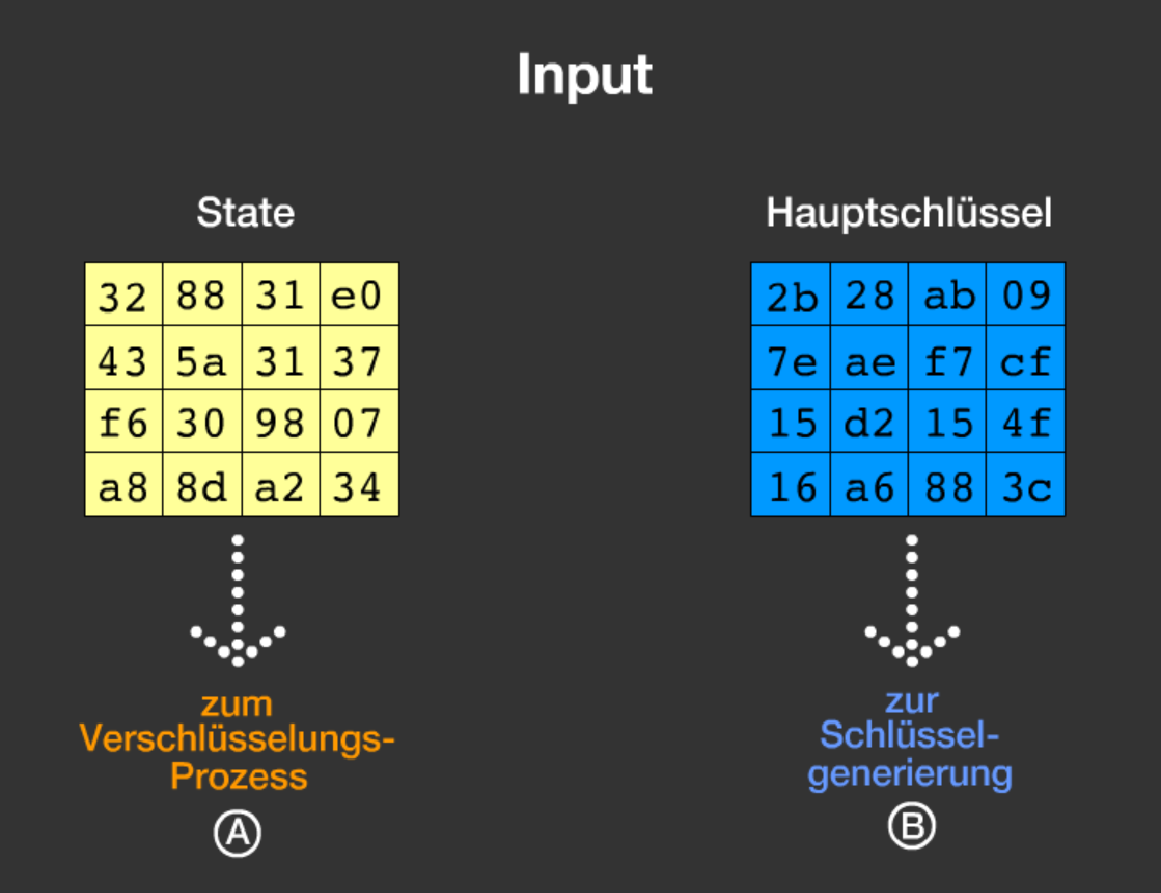
\includegraphics[scale=0.6]{figures/AES-Visualization-Zabala-Flash-step3_de}
\caption{AES-Visualisierung von Enrique Zabala aus CT1 (Teil 1)}
\label{AES-Visualization-Zabala-Flash-step3}
\end{center}
\end{figure}

\begin{figure}[!ht]
\begin{center}
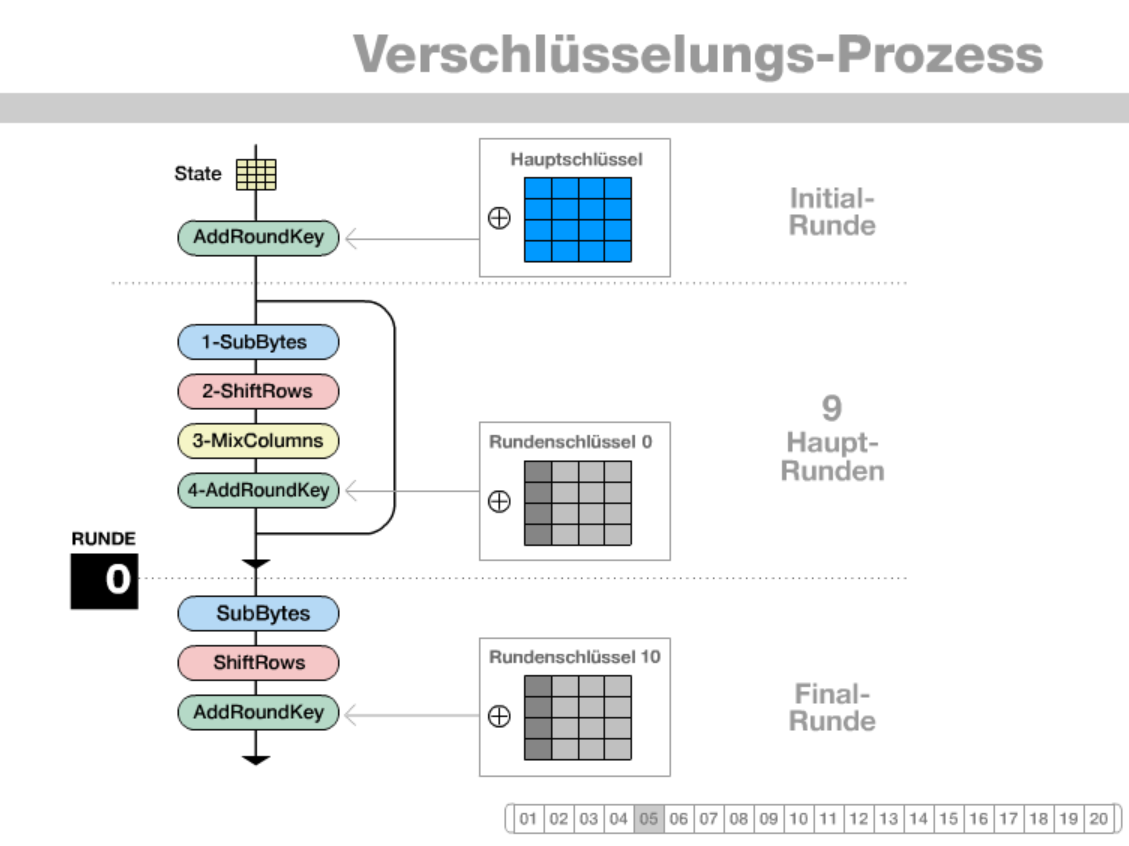
\includegraphics[scale=0.6]{figures/AES-Visualization-Zabala-Flash-step5_de}
\caption{AES-Visualisierung von Enrique Zabala aus CT1 (Teil 2)}
\label{AES-Visualization-Zabala-Flash-step5}
\end{center}
\end{figure}
%\end{sloppypar}


\clearpage
\noindent Im Folgenden wollen wir einen 128-bit-Block Klartext mit einem 128-bit
Schl�ssel mit AES im CBC-Modus verschl�sseln. Vom erhaltenen Geheimtext interessiert
uns nur der 1. Block (wenn mehr vorhanden ist, ist das Padding -- hier Null-Padding).
Zur Veranschaulichung machen wir das einmal mit CT2 und einmal mit OpenSSL.\\

\noindent Abbildung \ref{AES_Encrypting-one-block-with-CT2} zeigt die Verschl�sselung
eines Blocks in {\bf CT2}\index{CT2}.

\noindent Der Klartext \glqq AESTEST1USINGCT2\grqq~wird nach Hex
(41 45 53 54 45 53 54 31 55 53 49 4E 47 43 54 32)
konvertiert. Damit und mit dem Schl�ssel 3243F6A8885A308D313198A2E0370734
erzeugt die AES-Komponente dann den Geheimtext. Dieser lautet in Hex:\\
B1 13 D6 47 DB 75 C6 D8 47 FD 8B 92 9A 29 DE 08

\begin{figure}[ht]
\begin{center}
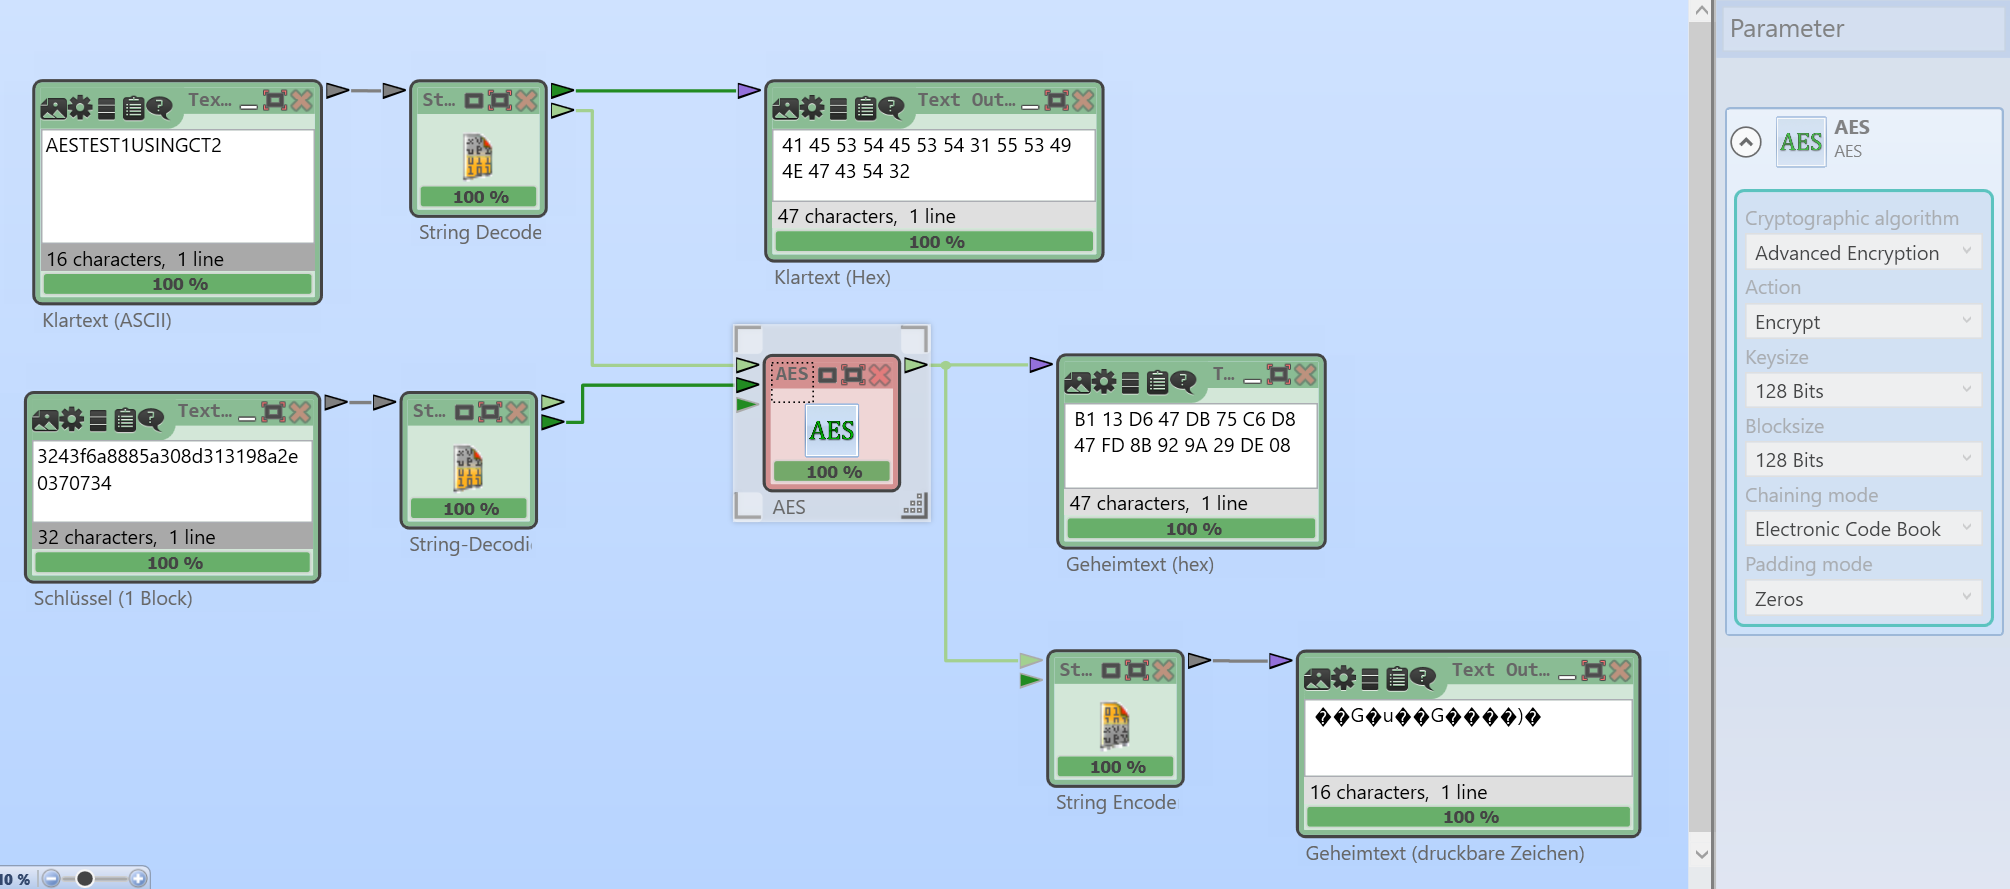
\includegraphics[scale=0.42]{figures/AES_Encrypting-one-block-with-CT2_de}
\caption{AES-Verschl�sselung (genau 1 Block ohne Padding) in CT2} 
\label{AES_Encrypting-one-block-with-CT2}
\end{center}
\end{figure}

\vspace{15pt}
\noindent Dasselbe Ergebnis kann man mit {\bf OpenSSL}\index{OpenSSL}%
\footnote{%
      OpenSSL\index{OpenSSL} ist eine sehr verbreitete freie Open-Source Kryptobibliothek,
      die von vielen Anwendungen benutzt wird, bspw. um das TLS-Protokoll zu implementieren.
      Zu OpenSSL geh�rt auch das Kommandozeilentool openssl, mit dem man die Funktionalit�t
      auf vielen Betriebssystemen direkt ausprobieren und Zertifikate beantragen, erzeugen
      und verwalten kann.\\
      Im Gegensatz zum ebenfalls sehr verbreiteten und sehr guten Kommandozeilentool gpg
      von GNU Privacy Guard\index{GnuPG}
      (\url{https://de.wikipedia.org/wiki/GNU_Privacy_Guard})
      erlaubt openssl auch Aufrufe, die sehr ins Detail gehen.
      Bei gpg liegt der Schwerpunkt auf den im praktischen Einsatz befindlichen Ciphersuites.
      Einfach genau einen Block ohne Padding zu verschl�sseln geht unseres Wissens mit dem
      Kommandozeilentool gpg nicht.\\
      Siehe auch \url{https://de.wikipedia.org/wiki/OpenSSL}.
%      Also see \url{https://en.wikipedia.org/wiki/OpenSSL}.
  }
auf der Kommandozeile auf ff. Weise erzielen:
\begin{opensslcode}
\begin{Verbatim}%
[fontsize=\footnotesize]
>openssl enc -e -aes-128-cbc
        -K 3243F6A8885A308D313198A2E0370734
        -iv 00000000000000000000000000000000
        -in klartext-1.hex  -out klartext-1.hex.enc
>dir
06.07.2016  12:43                16 key.hex
20.07.2016  20:19                16 klartext-1.hex
20.07.2016  20:37                32 klartext-1.hex.enc
\end{Verbatim}
\caption{AES-Verschl�sselung (von genau einem Block ohne Padding) in OpenSSL}
\label{cm_AES_no-padding:OpenSSL_example}
\end{opensslcode}





\clearpage
% HACK to fix warning "destination with the same identifier .. has already been used, ...":
% REMOVED, because it caused missing index entries
%\makeatletter \renewcommand{\thepage}{\csname @arabic\endcsname \c@page} \makeatother
% --------------------------------------------------------------------------
\subsubsection{Ergebnisse zur theoretischen Kryptoanalyse von AES}
\label{cm_New-AES-Analysis}
\index{Kryptoanalyse}
\index{AES}

Im Anschluss finden Sie einige Informationen, die das AES-Verfahren in
letzter Zeit in Zweifel zogen -- unserer Ansicht nach aber (noch)
unbegr�ndet. Die folgenden Informationen beruhen vor allem auf den unten
angegebenen Originalarbeiten und auf \cite{Wobst2002} und
\cite{Lucks2002}.

Der AES bietet mit einer Mindestschl�ssell�nge von 128 Bit gegen
Brute-Force-Angriffe auch auf l�ngere Sicht gen�gend Sicherheit -- es sei
denn, es st�nden entsprechend leistungsf�hige Quantencomputer zur
Verf�gung. Der AES war immun gegen alle bis dahin bekannten
Krypto"-analyse-Verfahren, die vor allem auf statistischen
�berlegungen beruhen und auf DES angewandt wurden: man konstruiert aus
Geheim- und Klartextpaaren Ausdr�cke, die sich nicht rein zuf�llig
verhalten, sondern R�ckschl�sse auf den verwendeten Schl�ssel zulassen.
Dazu waren aber unrealistische Mengen an abgeh�rten Daten n�tig.

Bei Kryptoverfahren bezeichnet man solche Kryptoanalyseverfahren als
"`akademischen Erfolg"' oder als "`kryptoanalytischen Angriff"', da sie
theoretisch schneller sind als das Durchprobieren aller Schl�ssel, das
beim Brute-Force-Angriff\index{Angriff!Brute-Force} verwendet wird. Im
Fall des AES mit maximaler Schl�ssell�nge (256 Bit) braucht die
ersch�pfende Schl�sselsuche im Durchschnitt $2^{255}$
Verschl�sselungsoperationen. Ein kryptoanalytischer Angriff muss diesen
Wert unterbieten. Als aktuell gerade noch praktikabel (z.B. f�r einen
Geheimdienst) gilt ein Aufwand von $2^{75}$ bis $2^{90}$
Verschl�sselungsoperationen.

Eine neue Vorgehensweise wurde in der Arbeit von Ferguson, Schroeppel
und Whiting im Jahre 2001 \cite{Ferguson2001} beschrieben: Sie stellten
AES als geschlossene Formel (in der Form einer Art Kettenbruch) dar,
was aufgrund seiner "`relativ"' �bersichtlichen Struktur gelang. Da
diese Formel aus rund 1 Billiarde Summanden besteht, taugt sie zun�chst
nicht f�r die Kryptoanalyse. Dennoch war die wissenschaftliche Neugier
geweckt. Bereits bekannt war, dass sich der 128-Bit-AES als ein
�berbestimmtes System von rund 8000 quadratischen Gleichungen
(�ber algebraischen Zahlk�rpern) mit rund 1600 Variablen (einige
Unbekannte sind die Schl�sselbits) darstellen l�sst -- solch gro�e
Gleichungssysteme sind praktisch nicht l�sbar. Dieses Gleichungssystem
ist relativ d�nn besetzt (\glqq sparse\grqq), d.h. von den insgesamt etwa
1.280.000 m�glichen quadratischen Termen tauchen nur relativ wenige
�berhaupt im Gleichungssystem auf.

Die Mathematiker Courtois und Pieprzyk \cite{Courtois2002} ver�ffentlichten 
2002 eine Arbeit, die in der Krypto-Szene stark diskutiert wird: Sie 
entwickelten das auf der Eurocrypt 2000 von Shamir et al. vorgestellte 
XL-Verfahren (eXtended Linearization) weiter zum XSL-Verfahren 
(eXtended Sparse Linearization). Das XL-Verfahren ist eine heuristische 
Technik, mit der es manchmal gelingt, gro�e nicht-lineare Gleichungssysteme 
zu l�sen und die bei der Analyse eines asymmetrischen Algorithmus (HFE) 
angewandt wurde.  Die Innovation von Courtois und Pieprzyk war, das 
XL-Verfahren auf symmetrische Verfahren anzuwenden: Das XSL-Verfahren kann
auf spezielle Gleichungssysteme angewandt werden. Damit k�nnte ein 
256-Bit-AES-Verfah"-ren in rund $2^{230}$ Schritten geknackt werden. Dies ist 
zwar immer noch ein rein akademischer Angriff, aber er ist richtungsweisend
f�r eine ganze Klasse von Blockchiffren. Das generelle Problem mit diesem
Angriff besteht darin, dass man bisher nicht angeben kann, unter welchen
Umst�nden er zum Erfolg f�hrt: die Autoren geben in ihrer Arbeit notwendige
Bedingungen an; es ist nicht bekannt, welche Bedingungen hinreichend sind.
Neu an diesem Angriff war erstens, dass dieser Angriff nicht auf Statistik,
sondern auf Algebra beruhte. Dadurch erscheinen Angriffe m�glich, die nur
geringe Mengen von Geheimtext brauchen. Zweitens steigt damit die Sicherheit
eines Produktalgorithmus%
\index{Produktalgorithmus}\index{Verschl�sselung!Produktalgorithmus}%
\footnote{%
Ein Geheimtext kann selbst wieder Eingabe f�r eine Chiffrierung sein. Eine
Mehrfachverschl�sselung (cascade cipher)
\index{Verschl�sselung!Mehrfachverschl�sselung}\index{Mehrfachverschl�sselung}
\index{Kaskaden}
entsteht aus einer Komposition von mehreren Verschl�sselungstransformationen.
Die Gesamtchiffrierung wird Produktalgorithmus oder Kaskadenalgorithmus
genannt (manchmal ist die Namensgebung abh�ngig davon, ob die verwendeten
Schl�ssel statistisch abh�ngig oder unabh�ngig sind).\\
Nicht immer wird die Sicherheit eines Verfahrens durch Produktbildung 
erh�ht.\\
Dieses Vorgehen wird auch {\em innerhalb} moderner Algorithmen angewandt:
Sie kombinieren in der Regel einfache und, f�r sich genommen, kryptologisch
relativ unsichere Einzelschritte in mehreren Runden zu einem leistungsf�higen
Gesamtverfahren. Die meisten modernen Blockchiffrierungen (z.B. DES, IDEA)
sind Produktalgorithmen.\\
Als Mehrfachverschl�sselung wird auch das Hintereinanderschalten desselben
Verfahrens mit verschiedenen Schl�sseln wie bei Triple-DES bezeichnet.\index{DES!Triple-DES}
}
nicht mehr exponentiell mit der Rundenzahl.

Aktuell wird sehr intensiv auf diesem Gebiet geforscht: z.B. stellten
Murphy und Robshaw auf der Crypto 2002 ein Papier vor \cite{Robshaw2002a},
das die Kryptoanalyse drastisch verbessern k�nnte: Der Aufwand f�r
128-Bit-Schl�ssel wurde auf $2^{100}$ gesch�tzt, indem sie AES als
Spezialfall eines Algorithmus BES (Big Encryption System) darstellten,
der eine besonders "`runde"' Struktur hat. Aber auch $2^{100}$
Rechenschritte liegen jenseits dessen, was praktisch in absehbarer Zeit
realisierbar ist. Bei 256 Bit Schl�ssell�nge sch�tzen die Autoren
den Aufwand f�r den XSL-Angriff auf $2^{200}$ Operationen.

Weitere Details finden Sie unter den Weblinks bei
\hyperlink{CM_HT_Weblink_Rijndael-Cryptosystem}{\glqq Das AES-/Rijndael-Kryptosystem\grqq}.
% nur \href oder \url r�ckt nicht ein, deshalb \item dazu !
%\vspace{-10pt}
%\begin{itemize}
%  \item[] \url{http://www.cryptosystem.net/aes} \\
%          \url{http://www.minrank.org/aes/} 
%\end{itemize}


F�r AES-256 w�re der Angriff ebenfalls viel besser als
Brute-Force\index{Angriff!Brute-Force}, aber noch weit au�erhalb der
Reichweite realisierbarer Rechenpower.

\begin{sloppypar}
Die Diskussion ist z.Zt. sehr kontrovers: Don Coppersmith (einer der
DES-Erfinder) z.B. bezweifelt die generelle Durchf�hrbarkeit des Angriffs:
XLS liefere f�r AES gar keine L�sung \cite{Coppersmith2002}. Dann w�rde
auch die Optimierung von Murphy und Robshaw \cite{Robshaw2002b} nicht
greifen.
\end{sloppypar}

2009 ver�ffentlichten Biryukov und Khovratovich \cite{Biryukov2009} einen
weiteren theoretischen Angriff auf AES, der sich anderer Techniken bedient, als
die oben vorgestellten. Sie verwenden Methoden aus der Kryptoanalyse von
Hashfunktionen (lokale Kollisionen und das Boomerang-Verfahren) und
konstruierten daraus einen Related-Key-Angriff auf AES-256. D.~h.\ der Angreifer
muss nicht nur in der Lage sein, beliebige Daten zu verschl�sseln (chosen plain
text), sondern auch den ihm unbekannten Schl�ssel manipulieren k�nnen (related
key).

Unter diesen Angriffs-Voraussetzungen reduziert der Angriff den Aufwand, einen
AES-256-Schl�ssel zu ermitteln, auf eine (asymmetrische) Komplexit�t von
$2^{119}$ Zeit und $2^{77}$ Speicher. Bei AES-192 ist der Angriff noch weniger
praktikabel, f�r AES-128 geben die Autoren keinen Angriff an.


% --------------------------------------------------------------------------
\subsection{Algebraische oder algorithmische Kryptoanalyse symmetrischer Verfahren}
\index{Angriff!algebraisch}
\label{cm_Algebraic-versus-Symmetr}

Es gibt unterschiedliche moderne Angriffsverfahren, die die Strukturen eines Problems direkt oder nach einer Transformation des Problems angreifen. Eines dieser Angriffsverfahren beruht auf dem Erf�llbarkeitsproblem der Aussagenlogik (SAT, von englisch satisfiability)%
\footnote{%
 \url{http://de.wikipedia.org/wiki/Erf%C3%BCllbarkeitsproblem_der_Aussagenlogik}
}.


%\vskip +25 pt
\paragraph*{Beschreibung SAT-Solver}\index{SAT-Solver}\mbox{}
\hypertarget{ht_SAT-Solver}{}

Ein sehr altes und gut studiertes Problem in der Informatik ist das sogenannte SAT-Problem. Hier gilt es, f�r eine gegebene Boolesche Formel herauszufinden, ob es eine Belegung der Variablen gibt, so dass die Auswertung der Formel den Wert 1 ergibt. 

Beispiel: Die Formel \glqq A UND B\grqq~wird zu 1 ausgewertet, wenn A=B=1 gilt. F�r die Formel \glqq A UND NICHT(A)\grqq~gibt es keine Belegung f�r A, so dass sie zu 1 ausgewertet wird.

F�r gr��ere Formeln ist es nicht so einfach herauszufinden, ob eine Formel zu 1 ausgewertet werden kann (dieses Problem geh�rt zu den NP-vollst�ndigen Problemen). Daher wurden spezielle Tools entwickelt, um dieses Problem f�r generelle Boolesche Formeln zu l�sen, sogenannte SAT-Solver\footnote{
    Mit {\bf CT2}\index{CT2} k�nnen Sie im Startcenter
    �ber {\bf Vorlagen \textbackslash{} Mathematisch \textbackslash{}
    SAT-Solver (Texteingabe)}  und  {\bf SAT-Solver (Dateieingabe)} einen
    SAT-Solver aufrufen.
    }. Wie sich herausgestellt hat, k�nnen SAT-Solver auch eingesetzt werden, um Krypto-Verfahren
anzugreifen.


%\vskip +25 pt
\paragraph*{SAT-Solver basierte Kryptoanalyse}\index{SAT-Solver}\mbox{}
\hypertarget{ht_SAT-Solver_Cryptanalysis}{}

Der generelle Ansatz, um SAT-Solver in der Kryptoanalyse einzusetzen, ist sehr einfach: Zun�chst wird das kryptographische Problem, etwa das Finden des symmetrischen Schl�ssels oder die Umkehrung einer Hashfunktion, in ein SAT-Problem �bersetzt. Dann wird ein SAT-Solver verwendet, um eine L�sung f�r das SAT-Problem zu finden. Die L�sung des SAT-Problems l�st dann auch das urspr�ngliche kryptographische Problem.
Der Artikel von Massacci \cite{Massacci2000} beschreibt die erste bekannte Verwendung eines SAT-Solvers in diesem Kontext. Leider stellte sich sehr bald heraus, dass ein solch genereller Ansatz in der Praxis nicht effizient eingesetzt werden kann. Die kryptographischen SAT-Probleme sind sehr komplex und die Laufzeit eines SAT-Solvers w�chst exponentiell mit der Problemgr��e. Daher werden in modernen Ans�tzen SAT-Solver nur f�r das L�sen von Teilproblemen der Kryptoanalyse verwendet. Ein gutes Beispiel zeigt der Artikel von Mironov und Zhang \cite{Mironov2006}. Hier wird anhand eines Angriffs auf Hashfunktionen gezeigt, zur L�sung welcher Teilprobleme SAT-Solver effizient eingesetzt werden k�nnen.

% Todo later: xxxxxxxxx Bsp aus CT2.1 erg�nzen mit SAT-Analyzer (nicht nur SAT-Solver)
%             Erfordert wahrscheinlich den CT2-Store, da es vorerst nur mit cygwin l�uft.
% \index{ZZZ6b-xxxxxxxxxxxxxxxx-Bsp aus CT2.1 ergaenzen} 
% \index{ZZZ6b-xxxxxxxxxxxxxxxxD}




% --------------------------------------------------------------------------
\subsection{Aktueller Stand der Brute-Force-Angriffe auf symmetrische Verfahren}
\index{Angriff!Brute-Force}
\index{RC5}
\label{cm_Brute-force-versus-Symmetr}

Anhand der Blockchiffre RC5 kann der aktuelle Stand von Brute-Force-Angriffen
auf symmetrische Verschl�sselungsverfahren gut erl�utert werden.

\begin{sloppypar}
Als Brute-Force-Angriff (exhaustive search, trial-and-error) bezeichnet
man das vollst�ndige Durchsuchen des Schl�sselraums: Dazu m�ssen
keine besonderen Analysetechniken eingesetzt werden. Stattdessen wird
der Geheimtext mit allen m�glichen Schl�sseln des Schl�sselraums
entschl�sselt%
\footnote{%
  Mit CT1\index{CT1} k�nnen Sie �ber das Men�
  {\bf Analyse \textbackslash{} Symmetrische Verschl�sselung (modern)}
  ebenfalls Brute-Force-Analysen von modernen symmetrischen Verfahren
  durchf�hren (unter der schw�chsten aller m�glichen Annahmen: Der
  Angreifer kennt nur den Geheimtext, er f�hrt also einen
  Ciphertext-only-Angriff durch).\\
  Mit CT2\index{CT2} k�nnen Sie bei den Vorlagen unter
  {\bf Kryptoanalyse \textbackslash{} Modern} ebenfalls Brute-Force-Analysen
  durchf�hren. Besonders m�chtig ist die KeySearcher-Komponente, die
  die Ausf�hrung auch auf mehrere Rechner verteilen kann.
}
und gepr�ft, ob der resultierende Text einen sinnvollen
Klartext ergibt%
\footnote{%
  Ist der Klartext nat�rlich-sprachlich und wenigstens 100 B lang, kann
  diese Pr�fung ebenfalls automatisiert durchgef�hrt werden.\\
  Um in einer sinnvollen Zeit auf einem Einzel-PC ein Ergebnis zu
  erhalten, sollten Sie nicht mehr als 24 Bit des Schl�ssels als
  unbekannt kennzeichnen.}.
Bei einer Schl�ssell�nge von 64 Bit sind dies maximal
$2^{64}$ = 18.446.744.073.709.551.616 oder rund 18 Trillionen zu
�berpr�fende Schl�ssel\index{CrypTool}.
\end{sloppypar}

Um zu zeigen, welche Sicherheit bekannte symmetrische Verfahren wie
DES, Triple-DES oder RC5\index{DES}\index{RC5}\index{DES!Triple-DES}
haben, veranstaltete z.B. RSA Security
sogenannte Cipher-Challenges\index{Challenge}.\footnote{%
  \url{https://www.emc.com/emc-plus/rsa-labs/historical/the-rsa-laboratories-secret-key-challenge.htm}\\
  Im Mai 2007 meldete RSA Inc leider, dass sie die Korrektheit der bis dahin
  nicht gel�sten RC5-72 Challenge nicht best�tigen werden.

  Cipher-Challenges gibt es auch f�r asymmetrische Verfahren
  (siehe Kapitel \ref{nt:NoteFactorization}).

  Ein weites Spektrum einfacher und komplexer, symmetrischer und asymmetrischer
  R�tsel-Aufgaben bietet der internationale Krypto-Wettbewerb
  {\bf MysteryTwister C3}: %% \glqq MysteryTwister C3\grqq:
  \url{http://www.mysterytwisterc3.org}.
  \index{MTC3}\index{Krypto-Wettbewerb}
  }
Unter kontrollierten Bedingungen wurden Preise ausgelobt, um Geheimtexte
(verschl�sselt mit verschiedenen Verfahren und verschiedenen
Schl�ssell�ngen) zu entschl�sseln und den symmetrischen Schl�ssel
zu ermitteln. Damit werden theoretische Resultate praktisch best�tigt.

Dass das "`alte"' Standard-Verfahren DES mit der fixen Schl�ssell�nge
von 56 Bit nicht mehr sicher ist, wurde schon im Januar 1999 von der
Electronic Frontier Foundation (EFF) demonstriert, als sie mit Deep Crack
eine DES-verschl�sselte Nachricht in weniger als einem Tag
knackten.\footnote{%
  \url{https://www.emc.com/emc-plus/rsa-labs/historical/des-challenge-iii.htm}
}

Der aktuelle Rekord f�r starke symmetrische Verfahren liegt bei 64 Bit
langen Schl�sseln. Dazu wurde das Verfahren RC5 benutzt, eine
Blockchiffre mit variabler Schl�ssell�nge. 

Die RC5-64 Challenge wurde im Juli 2002 nach 5 Jahren vom
distributed.net-Team gel�st.\footnote{%
 \url{http://www.distributed.net/Pressroom_press-rc5-64}\\
 \url{http://www.distributed.net/images/9/92/20020925_-_PR_-_64_bit_solved.pdf}
}
Insgesamt arbeiteten 331.252 Personen gemeinsam �ber das Internet
zusammen.\footnote{%
Eine �bersicht �ber die aktuellen Projekte zum verteilten Rechnen finden
Sie unter:\\
\url{http://distributedcomputing.info/}
}
Ge"-testet wurden rund 15 Trillionen Schl�ssel, bis der
richtige Schl�ssel gefunden wurde.%
\footnote{%
  CT2\index{CT2} hat begonnen, mit einer allgemeinen Infrastruktur f�r verteiltes
  Rechnen zu experimentieren (CrypCloud\index{CrypCloud}, die sowohl Peer-to-Peer
  als zentralisiert eingesetzt werden kann). Damit wird CT2 in der Zukunft in die
  Lage versetzt, Berechnungen auf viele Computer zu verteilen.
  Was man erreichen kann, wenn die Komponenten f�r die Parallelisierung eingerichtet
  sind, zeigte ein Cluster zur verteilten Kryptoanalyse von DES und AES:
  Stand 21. M�rz 2016 funktionierte ein Brute-force-Angriff (verteilte Schl�sselsuche)
  gegen AES auf 50 i5-PCs, jeder mit 4 virtuelles CPU-Kernen. Diese 200 virtuellen
  \glqq Worker Threads\grqq~konnten ca. 350 Millionen AES-Schl�ssel/sec testen. Die
  \glqq Cloud\grqq~verarbeitete dabei insgesamt ca. 20 GB/sec an Daten. CrypCloud
  ist eine Peer-to-Peer-basierte Cloud, so dass CT2-Nutzer sich freiwillig bei
  verteilten Jobs anschlie�en k�nnen.
}


Somit sind symmetrische Verfahren (auch wenn sie keinerlei
kryptographische Schw�"-chen haben) mit 64 Bit langen Schl�sseln
keine geeigneten Verfahren mehr sind, um sensible Daten l�nger geheim
zu halten.




% --------------------------------------------------------------------------
\newpage
\section[Asymmetrische Verschl�sselung] % Was zw. [..] steht, kommt ins Inhaltsverzeichnis!
{Asymmetrische Verschl�sselung\footnotemark}
  \footnotetext{%
   Das RSA-Kryptosystem kann mit CT1\index{CT1} �ber das Men� 
   {\bf Einzelverfahren \textbackslash{} RSA-Kryptosystem \textbackslash{} 
   RSA-Demo} in vielen Variationen nachvollzogen werden.\\
   Mit CT1\index{CT1} k�nnen Sie �ber das Men�
   {\bf Ver-/Entschl�sseln \textbackslash{} Asymmetrisch} mit RSA 
   ver- und entschl�sseln. In beiden F�llen m�ssen Sie ein 
   RSA-Schl�sselpaar ausw�hlen. Nur bei der Entschl�sselung wird der 
   geheime RSA-Schl�ssel ben�tigt -- deshalb wird nur hier die PIN abgefragt.\\
   Mit CT2\index{CT2} k�nnen Sie bei den Vorlagen unter
   {\bf Kryptographie \textbackslash{} Modern} ebenfalls asymmetrische
   Verfahren durchf�hren.\\
   JCT\index{JCT} bietet asymmetrische Verfahren wie RSA sowohl im
   Men� {\bf Visualisierungen} der Standard-Perspektive als auch in der
   Algorithmen-Perspektive.%Funktionalen
  }
\label{cm_Section_Asymmetric-encryption}

Bei der {\em asymmetrischen} Verschl�sselung
\index{Verschl�sselung!asymmetrisch} hat jeder Teilnehmer 
ein pers�nliches Schl�sselpaar, % Schl�s\-selpaar, be_24.5.03: so vorher und kam auch richtig raus! 
das aus einem {\em geheimen} \index{Schl�ssel!geheim} und einem 
{\em �ffentlichen} Schl�ssel \index{Schl�ssel!�ffentlich} besteht.
Der �ffentliche Schl�ssel wird, der Name deutet es an,
�ffentlich bekanntgemacht -- zum Beispiel in einem Schl�sselverzeichnis
im Internet (diese Art von \glqq Schwarzem Brett\grqq~wird auch Directory oder
�ffentlicher Schl�sselring genannt) oder in einem sogenannten \index{Zertifikat} Zertifikat.
\par \vskip + 3pt

Die asymmetrische Verschl�sselung veranschaulicht Abbildung \ref{cm_Figure_Asymmetric-Enc_Public-Key-Enc}:
\begin{figure}[ht]
\begin{center}
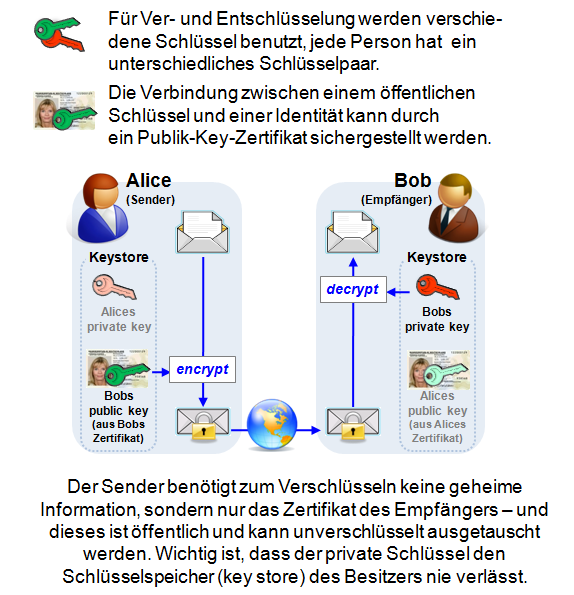
\includegraphics[scale=0.7]{figures/AsymmetricEnc_Figure_Chap1_de.png}
\caption{Asymmetrische oder Public-Key-Verschl�sselung} 
\label{cm_Figure_Asymmetric-Enc_Public-Key-Enc}
\end{center}
\end{figure}

M�chte Alice\index{Alice}%
\footnote{%
  Zur Beschreibung kryptographischer Protokolle werden den Teilnehmern
  oft Namen gegeben (vergleiche \cite[S. 23]{Schneier1996}). 
  Alice und Bob\index{Bob} f�hren alle allgemeinen 2-Personen-Protokolle durch,
  wobei Alice dies initiiert und Bob antwortet.
  Die Angreifer werden als Eve (eavesdropper = passiver Lauscher) und
  Mallory (malicious active attacker = b�swilliger, aktiver Abgreifer)
  bezeichnet.
  }
mit Bob kommunizieren, so sucht sie Bobs �ffentlichen Schl�ssel
und benutzt ihn, um ihre Nachricht an ihn zu
verschl�sseln. Diesen verschl�sselten Text schickt sie dann an Bob,
der mit Hilfe seines geheimen Schl�ssels den Text wieder entschl�s"-seln
kann. Da einzig Bob Kenntnis von seinem geheimen Schl�ssel hat, ist
auch nur er in der Lage, an ihn adressierte Nachrichten zu
entschl�sseln.
Selbst Alice als Absenderin der Nachricht kann aus der von ihr
versandten (verschl�sselten) Nachricht den Klartext nicht wieder
herstellen. Nat�rlich muss sichergestellt sein, dass man aus dem
�ffentlichen Schl�ssel nicht auf den geheimen Schl�ssel schlie�en
kann.\par \vskip + 3pt

% Abbildung evtl. besser hier, wenn Seitenaufteilung ausginge.

Veranschaulichen kann man sich ein solches Verfahren mit einer
Reihe von einbruchssicheren Briefk�sten. Wenn ich eine Nachricht
verfasst habe, so suche ich den Briefkasten\index{Briefkasten} mit dem
Namensschild des Empf�ngers und werfe den Brief dort ein. Danach kann ich die
Nachricht selbst nicht mehr lesen oder ver�ndern, da nur der
legitime Empf�nger im Besitz des Schl�ssels f�r den Briefkasten
ist.\par \vskip + 3pt

Vorteil von asymmetrischen Verfahren ist das einfachere
\index{Schl�sselmanagement} Schl�sselmanagement. Betrachten wir
wieder ein Netz mit $n$ Teilnehmern. Um sicherzustellen, dass
jeder Teilnehmer jederzeit eine verschl�sselte Verbindung zu
jedem anderen Teilnehmer aufbauen kann, muss jeder Teilnehmer ein
Schl�sselpaar besitzen. Man braucht also $2n$ Schl�ssel oder $n$
Schl�sselpaare. Ferner ist im Vorfeld einer �bertragung kein
sicherer Kanal notwendig, da alle Informationen, die zur Aufnahme
einer vertraulichen Kommunikation notwendig sind, offen
�bertragen werden k�nnen. Hier ist lediglich%
\footnote{%
Dass auch dies nicht trivial ist, wird z.B. in Kapitel \ref{nt_Shared-Primes}
erl�utert.
Neben den Anforderungen bei der Schl�sselgenerierung ist zu beachten, dass
inzwischen auch die (Public-Key-)Infrastrukturen selbst Ziel von 
Cyber-Angriffen sind.
}
auf die Unverf�lschtheit (Integrit�t und Authentizit�t)
\index{Authentizit�t} des �ffentlichen Schl�ssels zu achten.
Nachteil: Im Vergleich zu symmetrischen Verfahren sind reine
asymmetrische Verfahren jedoch um ein Vielfaches langsamer.\par \vskip + 3pt

Das bekannteste asymmetrische Verfahren ist der \index{RSA} 
RSA-Algorithmus\index{CrypTool}%
\footnote{%
  RSA wird in diesem Skript ab Kapitel \ref{rsabeweis} ausf�hrlich beschrieben.
  Die aktuellen Forschungsergebnisse im Umfeld von RSA werden in Kapitel
  \ref{SecurityRSA} beschrieben.
}%
, der nach seinen Entwicklern Ronald \index{Rivest, Ronald} Rivest, 
Adi \index{Shamir, Adi} Shamir und Leonard \index{Adleman, Leonard} Adleman
benannt wurde. Der RSA-Algorith"-mus wurde 1978 ver�ffentlicht.\footnote{%
  Hinweise zur Geschichte von RSA und seiner Ver�ffentlichung, die nicht im Sinne
  der NSA war, finden sich in der Artikelserie {\em RSA \& Co. in der Schule:
  Moderne Kryptologie, alte Mathematik, raffinierte Protokolle}.
  Siehe \cite{Witten2006}, S. 55 ff (\glqq Penible L�mmergeier\grqq).
  \index{RSA \& Co. in der Schule}
}
Das Konzept der asymmetrischen Verschl�sselung wurde erstmals
von Whitfield Diffie \index{Diffie, Whitfield}  und 
Martin \index{Hellman, Martin} Hellman in Jahre 1976 vorgestellt. 
Heute spielen auch die Verfahren nach
ElGamal \index{ElGamal, Tahir} eine bedeutende Rolle, vor allem die
\index{Schnorr, Claus-Peter} Schnorr-Varianten im \index{DSA} DSA (Digital
\index{Signatur!digital}\index{DSA-Signatur}\index{Signatur!DSA}
Signature Algorithm).

\noindent Angriffe gegen asymmetrische Verfahren werden behandelt in\\
- Kapitel~ \ref{Chapter_ElementaryNT}: \hyperlink{Chapter_ElementaryNT}{Elementare Zahlentheorie},\\
- Kapitel~ \ref{Chapter_ModernCryptography}:
  \hyperlink{Chapter_ModernCryptography}{Moderne Kryptographie},\\
- Kapitel~ \ref{Chapter_EllipticCurves}:
  \hyperlink{Chapter_EllipticCurves}{Elliptische Kurven} und\\
- Kapitel \ref{Chapter_Dlog-FactoringDead}: \hyperlink{Chapter_Dlog-FactoringDead}
  {Aktuelle Resultate zum L�sen diskreter Logarithmen und zur Faktorisierung}.



% --------------------------------------------------------------------------
\newpage
\section[Hybridverfahren]{Hybridverfahren\footnotemark} 
\footnotetext{%
   In CT1\index{CT1} finden Sie dieses Verfahren �ber das Men�
   {\bf Ver-/Entschl�sseln \textbackslash{} Hybrid}:
   Dabei k�nnen Sie die einzelnen Schritte und ihre Abh�ngigkeiten mit konkreten
   Zahlen nachvollziehen. Die Variante mit RSA als asymmetrischem Verfahren
   ist graphisch visualisiert; die Variante mit ECC nutzt die Standard-Dialoge.
   In beiden F�llen wird AES als symmetrisches Verfahren eingesetzt.\index{AES}\\
   JCT\index{JCT} bietet Hybrid-Verfahren (z.B. ECIES) in der
   Algorithmen-Perspektive an unter {\bf Algorithms \textbackslash{} Hybrid Ciphers}.
}
\label{CM_Hybrid-procedures}
\index{Hybridverfahren}

Um die Vorteile von symmetrischen und asymmetrischen Techniken gemeinsam 
nutzen zu k�nnen, werden (zur Verschl�sselung) in der Praxis meist 
Hybridverfahren \index{Verschl�sselung!hybrid} verwendet.\par \vskip + 3pt

Hier werden die Mengen-Daten mittels symmetrischer Verfahren
verschl�sselt: Der Schl�ssel ist ein vom Absender zuf�llig\footnote{%
   Die Erzeugung zuf�lliger Zahlen\index{Zufall} ist ein wichtiger Bestandteil 
   kryptographisch sicherer Verfahren.\\
   - Mit CT1\index{CT1} k�nnen Sie �ber das Men�
   {\bf Einzelverfahren \textbackslash{} Zufallsdaten erzeugen}
   verschiedene Zufallszahlengeneratoren\index{Zufallsgenerator} (PRNGs) ausprobieren.
   �ber das Men� {\bf Analyse \textbackslash{} Zufallsanalyse} k�nnen Sie
   verschiedene Testverfahren f�r Zufallsdaten auf bin�re Dokumente
   anwenden.\\
   % CT1 konzentriert sich auf kryptographisch starke
   % {\bf Pseudo}zufallszahlengeneratoren. \glqq Echte\grqq~
   % Zufallsquellen werden nur �ber den Aufruf des Secude-Generators einbezogen.\\
   %
   - In CT2\index{CT2} k�nnen Sie im Startcenter
   mit dem Suchstring \glqq Zufall\grqq~Vorlagen (Templates) finden, die
   Zufallsgeneratoren\index{Zufallsgenerator} (PRNGs)
   nutzen. Die PRNGs nutzen intern bspw. Keccak\index{Keccak} oder den
   Linear Congruential Generator (LCG)\index{LCG}. Sie werden dann
   bspw. f�r Schl�sselgenerierung oder Dezimalisierung genutzt.\\
   %
   - JCT\index{JCT} bietet {\bf Pseudo}zufallszahlengeneratoren sowohl
   im Men� {\bf Algorithms \textbackslash{} Random Number Generator} der
   Standard-Perspektive als auch in der Algorithmen-Perspektive an.
}\index{Zufall}
generierter geheimer Sitzungsschl�ssel (session key)\index{Session Key},
der nur f�r diese Nachricht verwendet wird.

Anschlie�end wird dieser Sitzungsschl�ssel mit Hilfe des asymmetrischen
Verfahrens verschl�sselt und zusammen mit der Nachricht an den Empf�nger
�bertragen.

Der Empf�nger kann den Sitzungsschl�ssel mit Hilfe seines geheimen
Schl�ssels bestimmen und mit diesem dann die Nachricht entschl�sseln.

Auf diese Weise profitiert man von dem bequemen Schl�sselmanagement\index{Schl�sselmanagement}
asymmetrischer Verfahren (mit �ffentlichem und privatem Schl�ssel), und
man profitiert von der Schnelligkeit symmetrischer Verfahren, um gro�e
Datenmengen zu verschl�sseln (mit den geheimen Schl�sseln).



% --------------------------------------------------------------------------
\newpage
% \vskip +40 pt

\begin{ctsquote}
    Ein altes Sprichwort, angeblich gepr�gt von der
    US National Security Agency (NSA), sagt:\\
    \glqq Angriffe werden immer besser, niemals schlechter.\grqq\\
    ``Attacks always get better; they never get worse.''
\caption[IETF]{IETF\footnotemark}
\end{ctsquote}
\addtocounter{footnote}{0}\footnotetext{%
  \url{http://tools.ietf.org/html/rfc4270}\index{IETF}\index{NSA}
  }

% --------------------------------------------------------------------------
\section[Kryptoanalyse und symmetrische Chiffren f�r Lehrzwecke]{Kryptoanalyse und symmetrische Chiffren f�r Lehrzwecke\footnotemark} 
\footnotetext{%
  Ein sehr guter Start in die Kryptoanalyse ist das Buch von Mark Stamp \cite{Stamp2007}.
  Ebenfalls gut, aber sehr high-level und nur bezogen auf die Analyse symmetrischer
  Blockchiffren ist der Artikel von Bruce Schneier \cite{Schneier2000}.\\
  Einige der Cipher-Challenges bei \glqq MysteryTwister C3\grqq~
  (\url{http://www.mysterytwisterc3.org}) sind ebenfalls gut f�r Lehrzwecke
  einsetzbar.\index{MTC3}\index{Krypto-Wettbewerb}
}
\label{CM_Analysis-SymCiphers-Educational}
\index{Kryptoanalyse}

Verglichen mit den auf der Zahlentheorie beruhenden Public-Key-Verschl�sselungsverfahren wie RSA, ist die Struktur von AES\index{AES} und den meisten anderen modernen symmetrischen Verschl�sse"-lungsverfahren (wie DES, IDEA oder Present) sehr komplex und kann nicht so einfach wie RSA\index{RSA} erkl�rt werden.

Deshalb wurden zu Lehrzwecken vereinfachte Varianten moderner
symmetrischer Verfahren entwickelt, um Einsteigern die M�glichkeit zu geben,
Ver- und Entschl�sselung von Hand zu lernen und ein besseres Verst�ndnis zu
gewinnen, wie die Algorithmen im Detail funktionieren.
Diese vereinfachten Varianten helfen auch, die entsprechenden
Kryptoanalyse-Methoden zu verstehen und anzuwenden.

Die bekanntesten Varianten sind SDES (Simplified DES)%
\footnote{
  Visualisierung: Macht man in CT2\index{CT2} einen Doppelklick auf den Titel der
  SDES-Komponente, ist in der Fullscreen-Ansicht
  % fullscreen
  % in der Fullscreen-Ansicht  %% das gab eine Zeile zuviel und r�ckte 1.7. weiter.
  zu sehen, wie die Bits der eingegebenen Daten durch den Algorithmus flie�en.
  Ein Screen\-shot dazu:
  \url{https://www.facebook.com/CrypTool2/photos/a.505204806238612.1073741827.243959195696509/597354423690316}
}
und S-AES (Simplified-AES) von Prof. Ed Schaefer und seinen Studenten%
\footnote{
    Siehe auch den Artikel \glqq Devising a Better Way to Teach and Learn
    the Advanced Encryption Standard\grqq~unter
    \url{http://math.scu.edu/~eschaefe/getfile.pdf}
    % be_2016-07-17: dead link /toter Link: http://www.scu.edu/cas/research/cryptography.cfm
},
und Mini-AES (siehe das Kapitel~\ref{CM_Sage_Mini-AES} \glqq \nameref{CM_Sage_Mini-AES}\grqq):

\index{DES}\index{DES!SDES}\index{IDEA}\index{AES!Mini-AES}\index{AES!S-AES}
\begin{itemize}

\item Edward F. Schaefer: {\em A Simplified Data Encryption Standard Algorithm} 
      \cite{Schaefer1996}.

\item Raphael Chung-Wei Phan: {\em Mini Advanced Encryption Standard (Mini-AES):
                                   A Testbed for Cryptanalysis Students} 
      \cite{Phan2002}.

\item Raphael Chung-Wei Phan: {\em Impossible differential cryptanalysis of Mini-AES} 
      \cite{Phan2003}.

\item Mohammad A. Musa, Edward F. Schaefer, Stephen Wedig:
      {\em A simplified AES algorithm and its linear and differential cryptanalyses} 
      \cite{Musa2003}.

\item Nick Hoffman: {\em A SIMPLIFIED IDEA ALGORITHM} 
      \cite{Hoffman2006}.

\item S. Davod. Mansoori, H. Khaleghei Bizaki: 
      {\em On the vulnerability of Simplified AES Algorithm Against Linear Cryptanalysis} 
      \cite{Mansoori2007}.

\end{itemize}



% --------------------------------------------------------------------------
\section{Weitere Informationsquellen}

Neben den anderen Kapiteln in diesem Skript, der umfangreichen Fachliteratur
und vielen Stellen im Internet enth�lt auch die Online-Hilfe aller 
CrypTool-Varianten\index{CrypTool} sehr viele weitere Informationen zu den 
einzelnen symmetrischen und asymmetrischen Verschl�sselungsverfahren.




% ---------------------------------------------------------------------------
% ---------------------------------------------------------------------------
\newpage
\hypertarget{CM_Appendix_SageCode}{}
\section{Anhang: Beispiele mit SageMath}
\label{CM_Sage_samples}
\index{SageMath!Programmbeispiele}

\noindent Der folgende Abschnitt enth�lt SageMath Source-Code, der sich auf den
Inhalt des Kapitels~\ref{CM_Analysis-SymCiphers-Educational}
(\glqq \nameref{CM_Analysis-SymCiphers-Educational}\grqq) bezieht.

Weitere Details zu in SageMath enthaltenen Kryptoverfahren (z.B. zum Simplified
Data Encryption Standard SDES) finden sich z.B. in der Diplomarbeit von Minh Van
Nguyen \cite{Nguyen2009b}.

% ---------------------------------------------------------------------------
\subsection{Mini-AES}
\label{CM_Sage_Mini-AES}
\index{AES!Mini-AES}

Das SageMath-Modul \texttt{crypto/block\_cipher/miniaes.py} enth�lt den Mini-AES, mit
dem Studenten die Funktionsweise moderner Blockchiffren untersuchen k�nnen.

Mini-AES, urspr�nglich vorgestellt von \cite{Phan2002}, ist eine vereinfachte
Variante des Advanced Encryption Standard (AES) f�r Ausbildungszwecke.

Wie man Mini-AES benutzt, ist ausf�hrlich in der SageMath Reference-Page beschrieben:
\begin{sloppypar} % N�tig, da sonst ein schwarzer Punkt
  \url{http://doc.sagemath.org/html/en/reference/cryptography/sage/crypto/block_cipher/miniaes.html}.
\end{sloppypar}

Das folgende SageMath-Code-Beispiel~\ref{cm_Mini-AES:Sage_example}
ist aus den Release-Notes von SageMath 4.1%
\footnote{
  Siehe \url{http://mvngu.wordpress.com/2009/07/12/sage-4-1-released/}.\\
  Weiterer Beispiel-Code zum Mini-AES findet sich in
  \cite[Kap. 6.5 und Anhang D]{Nguyen2009a}.
}
und ruft diese Implementierung des Mini-AES auf.


% Using [fontsize=\footnotesize,fontshape=tt] caused:
%   LaTeX Font Warning: Font shape `T1/cmtt/m/tt' undefined
%   (Font)              using `T1/cmtt/m/n' instead on input line 730.
% so deleted the fontshape parameter.
\begin{sagecode}
\begin{Verbatim}%
[fontsize=\footnotesize]
# We can encrypt a plaintext using Mini-AES as follows:
sage: from sage.crypto.block_cipher.miniaes import MiniAES
sage: maes = MiniAES()
sage: K = FiniteField(16, "x")
sage: MS = MatrixSpace(K, 2, 2)
sage: P = MS([K("x^3 + x"), K("x^2 + 1"), K("x^2 + x"), K("x^3 + x^2")]); P

[  x^3 + x   x^2 + 1]
[  x^2 + x x^3 + x^2]
sage: key = MS([K("x^3 + x^2"), K("x^3 + x"), K("x^3 + x^2 + x"), K("x^2 + x + 1")]); key

[    x^3 + x^2       x^3 + x]
[x^3 + x^2 + x   x^2 + x + 1]
sage: C = maes.encrypt(P, key); C

[            x       x^2 + x]
[x^3 + x^2 + x       x^3 + x]

# Here is the decryption process:
sage: plaintxt = maes.decrypt(C, key)
sage: plaintxt == P
True

# We can also work directly with binary strings:
sage: from sage.crypto.block_cipher.miniaes import MiniAES
sage: maes = MiniAES()
sage: bin = BinaryStrings()
sage: key = bin.encoding("KE"); key
0100101101000101
sage: P = bin.encoding("Encrypt this secret message!")
sage: C = maes(P, key, algorithm="encrypt")
sage: plaintxt = maes(C, key, algorithm="decrypt")
sage: plaintxt == P
True

# Or work with integers n such that 0 <= n <= 15:
sage: from sage.crypto.block_cipher.miniaes import MiniAES
sage: maes = MiniAES()
sage: P = [n for n in xrange(16)]; P
[0, 1, 2, 3, 4, 5, 6, 7, 8, 9, 10, 11, 12, 13, 14, 15]
sage: key = [2, 3, 11, 0]; key
[2, 3, 11, 0]
sage: P = maes.integer_to_binary(P)
sage: key = maes.integer_to_binary(key)
sage: C = maes(P, key, algorithm="encrypt")
sage: plaintxt = maes(C, key, algorithm="decrypt")
sage: plaintxt == P
True
\end{Verbatim}
\caption{Ver- und Entschl�sselung mit dem Mini-AES}
\label{cm_Mini-AES:Sage_example}
\end{sagecode}
\clearpage%% Um das Codebeispiel vor das ff. Kap. 1.8.2 zu bekommen.


% ---------------------------------------------------------------------------
\subsection{Weitere symmetrische Krypto-Algorithmen in SageMath}
\label{CM_Sage_SymCryptoAlg}

Die Referenz zu SageMath v7.2 f�hrt als kryptographische Funktionen u.a. auf:%
\footnote{
  Siehe 
  \url{http://doc.sagemath.org/html/en/reference/sage/crypto/index.html},\\
  \url{http://doc.sagemath.org/html/en/reference/cryptography/index.html} und\\
  \url{http://combinat.sagemath.org/doc/reference/cryptography/sage/crypto/stream.html}
}
\begin{itemize}
   \item Linear feedback shift register (LFSR),
   \item Blum-Blum-Shub (BBS): Pseudo-Zufallsbit-Generator (zu finden bei Streams),
   \item Gitter-basierte Funktionen.
% be_2016-07-17: Nicht mehr gefunden in Refrence 7.2:
% - ShrinkingGeneratorCryptosystem,
\end{itemize}



%------------------------------------------------------------------------------
\putbib[../de/references]
\addcontentsline{toc}{section}{Literaturverzeichnis}
\end{bibunit}

\noindent Alle Links wurden am 10.07.2016 �berpr�ft.



% --------------------------------------------------------------------------
\newpage
\chapter*{Web-Links}\addcontentsline{toc}{section}{Web-Links}

\begin{enumerate}

  \hypertarget{CM_HT_Weblink_Rijndael-Cryptosystem}{}
  \item \glqq AES Discussion Groups\grqq~beim NIST (archive page provided for historical purposes, last update on Feb 28th, 2001)\\
	% \grqq nach \item braucht die Tilde, aber kein weiteres Blank.
	%  Sonst reicht ein Blank, wenn ein weiteres Wort danach folgt
	%  (es reicht auch nicht, wenn danach ein Zeilenumbruch).
	\url{http://csrc.nist.gov/archive/aes/}

  \item Das AES-/Rijndael-Kryptosystem (page maintained by Nicolas T. Courtois, last update on Aug 24th, 2007)\\
        \url{http://www.cryptosystem.net/aes}

  \item distributed.net:~\glqq RC5-64 has been solved\grqq\\
        \url{http://www.distributed.net/Pressroom_press-rc5-64}

	% \begin{sloppypar}  ... \end{sloppypar} worked. Get rid of \\ before to avoid extra newline.
\item RSA Labs (ehemals RSA Security): ~\glqq The RSA Secret Key Challenge\grqq
        \begin{sloppypar}
	\url{https://www.emc.com/emc-plus/rsa-labs/historical/the-rsa-laboratories-secret-key-challenge.htm}
	\end{sloppypar}

  \item RSA Labs (ehemals RSA Security): ~\glqq DES Challenge\grqq\\
        \url{https://www.emc.com/emc-plus/rsa-labs/historical/des-challenge-iii.htm}

  \item Weiterf�hrende Links auf der CrypTool-Homepage\\
        \url{http://www.cryptool.org}
	       
\end{enumerate}

Alle Links wurden am 10.07.2016 �berpr�ft.



% Local Variables:
% TeX-master: "../script-de.tex"
% End:



\end{document}